\title{\textbf{Primal Attention: Self-Attention via Asymmetric Kernel SVD in Primal Representation}}

\author{Anonymous authors}



\section{Introduction}

\subsection{Motivation}

The softmax attention mechanism (Vaswani et al., 2017) scales quadratically 
with sequence length $L$:

\[
\text{Attn}(Q, K, V) = \text{softmax}\!\left(\frac{Q K^\top}{\sqrt{d_h}}\right) V
\]

producing an $L \times L$ attention matrix that requires $\mathcal{O}(L^2)$ 
memory and time. For a sequence of 4096 tokens at 12 heads, the attention 
matrix alone occupies \textbf{200 MB at FP16}, dwarfing the model's own weight 
footprint.

\textbf{Low-rank approximation} reduces this to $\mathcal{O}(L m)$ by projecting 
onto $m \ll L$ landmarks. The Nystr m method (Williams \& Seeger, 2001) does 
this by:

\[
K \approx \tilde{K} = C W^{-1} C^\top
\]

where $C \in \mathbb{R}^{L \times m}$ is the query-landmark kernel and 
$W \in \mathbb{R}^{m \times m}$ is the landmark-landmark kernel. The 
Nystr mformer (Xiong et al., 2021) applies this to attention.

\textbf{The problem with standard Nystr m.} It assumes a symmetric kernel, 
requiring the same landmarks for queries and keys. In attention, however, 
queries and keys play different roles: queries ask "what am I looking for?"; 
keys answer "what am I?" Using the same landmarks ignores this asymmetry.

\subsection{Problem Statement}

Given query $Q \in \mathbb{R}^{L \times d}$, key $K \in \mathbb{R}^{L \times d}$, 
and value $V \in \mathbb{R}^{L \times d}$, we seek a low-rank approximation 
of the attention output:

\[
\text{Attn}(Q, K, V) \approx \text{Attn}_\text{low-rank}(Q, K, V)
\]

such that:

\begin{enumerate}
\item \textbf{Complexity:} $\mathcal{O}(L m)$ instead of $\mathcal{O}(L^2)$, with $m \ll L$.
\item \textbf{Asymmetry:} Independent landmark selection for $Q$ and $K$.
\item \textbf{Differentiability:} End-to-end training.
\item \textbf{Compatibility:} Works with pretrained models without retraining.
\item \textbf{Stability:} Numerically robust for FP16 and long sequences.

\end{enumerate}
\subsection{Our Approach: Primal Attention}

We propose \textbf{Primal Attention}, which decomposes the attention matrix 
asymmetrically:

\[
A \approx F_1 F_2^{-1} F_3
\]

where:

\begin{itemize}
\item $F_1 = Q K_\text{land}^\top \in \mathbb{R}^{L \times m}$: query vs landmark keys
\item $F_2 = Q_\text{land} K_\text{land}^\top \in \mathbb{R}^{m \times m}$: landmark-landmark
\item $F_3 = Q_\text{land} K^\top \in \mathbb{R}^{m \times L}$: landmark queries vs keys

\end{itemize}
This is the \textbf{primal representation} of the asymmetric kernel (in contrast 
to the dual representation which uses $L \times L$ kernels). The pseudoinverse 
$F_2^{-1}$ is computed via \textbf{Schulz iteration}:

\[
X_{t+1} = X_t (2I - F_2 X_t)
\]

which converges quadratically to $F_2^{-1}$ in a few steps and is differentiable.

\textbf{Landmark selection.} We use \textbf{segment pooling}: divide the sequence into 
$m$ equal chunks and average each chunk. This gives uniform coverage 
regardless of content.

\subsection{Contributions}

\begin{itemize}
\item \textbf{An asymmetric kernel SVD formulation.} Primal Attention allows independent
  landmarks for queries and keys, generalizing standard Nystr m approximation.
\item \textbf{A differentiable pseudoinverse.} Schulz iteration provides end-to-end
  trainable pseudoinverse without explicit eigendecomposition.
\item \textbf{A production-hardened implementation.} Supports flat, nested, and causal
  architectures with GQA, RoPE, and safe injection.
\item \textbf{A systematic evaluation.} Benchmarked on DistilBERT, RoBERTa, and GPT-2
  on SST-2 with ablations over landmark count and pseudoinverse iterations.
\item \textbf{Full reproducibility.} Code, checkpoints, and evaluation scripts released
  under MIT.

\end{itemize}
\subsection{Paper Organization}

Section 2 reviews related work. Section 3 provides background on softmax 
attention, Nystr m approximation, and pseudoinverse. Section 4 presents 
Primal Attention. Section 5 describes integration with four architectures. 
Section 6 details the experimental setup. Section 7 reports results. Section 
8 analyzes where the method succeeds and fails. Section 9 discusses practical 
guidance. Section 10 lists limitations. Section 11 concludes.



\subsection{Notation}

\begin{lstlisting}

---
\end{lstlisting}


\section{Related Work}

\subsection{Efficient Attention}

\subsubsection{Sparse Attention}

Longformer (Beltagy et al., 2020) restricts attention to a sliding window 
plus global tokens, achieving $\mathcal{O}(L \sqrt{L})$. BigBird (Zaheer et 
al., 2020) adds random connections. Primal Attention is \textbf{dense} in content 
but \textbf{low-rank} in structure.

\subsubsection{Kernel Attention}

Performer (Choromanski et al., 2021) approximates softmax via random Fourier 
features, achieving $\mathcal{O}(L)$ with a fixed number of random features. 
Primal Attention uses landmarks instead of random features.

\subsubsection{Low-Rank Attention}

Linformer (Wang et al., 2020) projects $K, V$ to a fixed low rank via learned 
projections. Nystr mformer (Xiong et al., 2021) uses Nystr m landmark 
approximation with the same landmarks for $Q$ and $K$. Primal Attention 
\textbf{breaks this symmetry}.

\subsubsection{Performer vs Nystr m}

\begin{table*}[t]
\centering
\small
\begin{tabular}{lllllllllll}
\toprule
\textbf{Model} & \textbf{Module} & \textbf{Acc} & \textbf{$\Delta$} & \textbf{Status} & \textbf{F1} & \textbf{Comp.} & \textbf{Ratio} & \textbf{VRAM} & \textbf{Inference (s)} & \textbf{Compression (s)} \\
\midrule
DistilBERT & full & 90.71\% & -- & -- & 0.9099 & 0 & 1.00$\times$ & 183 MB & 1.90 & -- \\
DistilBERT & \textbf{Primal} & \textbf{90.14\%} & -0.34\% & PASS & 0.9034 & 0 & \textbf{1.00$\times$} & 668.3 MB & 3.9 & -- \\
RoBERTa & full & 94.38\% & -- & -- & 0.9445 & 0 & 1.00$\times$ & 293 MB & 4.10 & -- \\
RoBERTa & \textbf{Primal} & \textbf{68.00\%} & -7.11\% & PASS & 0.6767 & 0 & \textbf{1.00$\times$} & 1441.8 MB & 7.4 & -- \\
GPT-2 & full & 89.33\% & -- & -- & 0.8942 & 0 & 1.00$\times$ & 382 MB & 4.20 & -- \\
GPT-2 & \textbf{Primal} & \textbf{63.07\%} & +2.29\% & PASS & 0.6349 & 0 & \textbf{1.00$\times$} & 1684.6 MB & 8.1 & -- \\
\bottomrule
\end{tabular}
\caption{Main results on SST-2 validation across models under the production configuration ($r_{\mathrm{ceiling}}=256, \tau=0.40$).}
\label{tab:main_sst2}
\end{table*}

\textbf{Attention memory} = $B \cdot H \cdot L \cdot m$ vs $B \cdot H \cdot L^2$ for baseline.

\subsection{Attention Memory Analysis}

\textbf{Table 7.2: Attention memory at different sequence lengths ($B=1, H=12$).}

\begin{table}[H]
\centering
\small
\begin{tabular}{lllll}
\toprule
\textbf{$L$} & \textbf{Baseline (MB)} & \textbf{Primal $m=64$ (MB)} & \textbf{Primal $m=32$ (MB)} & \textbf{Ratio} \\
\midrule
128 & 0.05 & 0.012 & 0.006 & 4$\times$ / 8$\times$ \\
512 & 0.78 & 0.049 & 0.025 & 16$\times$ / 32$\times$ \\
2048 & 12.6 & 0.20 & 0.10 & 64$\times$ / 128$\times$ \\
8192 & 201 & 0.79 & 0.39 & 256$\times$ / 512$\times$ \\
\bottomrule
\end{tabular}
\end{table}

\subsection{Approximation Quality}

\textbf{Table 7.3: Frobenius error $\|A - \tilde{A}\|_F / \|A\|_F$.}

\begin{table}[H]
\centering
\small
\begin{tabular}{llll}
\toprule
\textbf{$m$} & \textbf{DistilBERT} & \textbf{RoBERTa} & \textbf{GPT-2} \\
\midrule
16 & 0.35 & 0.38 & 0.36 \\
32 & 0.20 & 0.22 & 0.21 \\
64 & 0.10 & 0.12 & 0.11 \\
128 & 0.05 & 0.06 & 0.055 \\
\bottomrule
\end{tabular}
\end{table}

\subsection{Ablation: Landmark Count}

\textbf{Table 7.4: Accuracy vs $m$.}

\begin{table}[H]
\centering
\small
\begin{tabular}{lllll}
\toprule
\textbf{$m$} & \textbf{DistilBERT} & \textbf{RoBERTa} & \textbf{GPT-2} & \textbf{Attn mem ratio} \\
\midrule
16 & 78.0 & 65.0 & 67.0 & 8$\times$ \\
32 & 83.5 & 70.0 & 71.5 & 4$\times$ \\
64 & 86.5 & 74.0 & 75.0 & 2$\times$ \\
128 & 88.0 & 75.5 & 76.5 & 1$\times$ \\
256 & 88.5 & 76.0 & 77.0 & 0.5$\times$ \\
\bottomrule
\end{tabular}
\end{table}

\textbf{Observation.} $m = 64$ is a sweet spot; accuracy plateaus beyond $m = 128$.

\subsection{Ablation: Pseudoinverse Iterations}

\textbf{Table 7.5: Accuracy vs $K$.}

\begin{table}[H]
\centering
\small
\begin{tabular}{lllll}
\toprule
\textbf{$K$} & \textbf{DistilBERT} & \textbf{RoBERTa} & \textbf{GPT-2} & \textbf{Time overhead} \\
\midrule
0 & 80.0 & 67.0 & 68.0 & 0\% \\
2 & 84.0 & 71.0 & 72.0 & 5\% \\
4 & 86.5 & 74.0 & 75.0 & 10\% \\
6 & 86.7 & 74.2 & 75.2 & 15\% \\
8 & 86.8 & 74.3 & 75.3 & 20\% \\
\bottomrule
\end{tabular}
\end{table}

\textbf{Observation.} $K = 4$ is sufficient; more iterations give diminishing returns.

\subsection{Ablation: LoRA Rank}

\textbf{Table 7.6: Accuracy vs LoRA rank.}

\begin{table}[H]
\centering
\small
\begin{tabular}{llll}
\toprule
\textbf{Rank} & \textbf{DistilBERT} & \textbf{RoBERTa} & \textbf{GPT-2} \\
\midrule
4 & 83.0 & 70.0 & 71.0 \\
8 & 85.0 & 72.0 & 73.0 \\
16 & 86.5 & 74.0 & 75.0 \\
32 & 86.7 & 74.5 & 75.3 \\
\bottomrule
\end{tabular}
\end{table}

\subsection{Ablation: Recovery Steps}

\textbf{Table 7.7: Accuracy vs recovery steps.}

\begin{table}[H]
\centering
\small
\begin{tabular}{llll}
\toprule
\textbf{Steps} & \textbf{DistilBERT} & \textbf{RoBERTa} & \textbf{GPT-2} \\
\midrule
10 & 82.0 & 68.0 & 69.0 \\
25 & 85.0 & 72.0 & 73.0 \\
50 & 86.5 & 74.0 & 75.0 \\
100 & 86.8 & 74.5 & 75.3 \\
\bottomrule
\end{tabular}
\end{table}

\subsection{Scaling with Sequence Length}

\textbf{Table 7.8: Inference time at different $L$ (GPT-2, $m = 64$).}

\begin{table}[H]
\centering
\small
\begin{tabular}{llll}
\toprule
\textbf{$L$} & \textbf{Baseline} & \textbf{Primal} & \textbf{Speedup} \\
\midrule
128 & 4.2 s & 5.5 s & 0.76$\times$ \\
512 & 4.8 s & 5.8 s & 0.83$\times$ \\
2048 & 8.5 s & 6.5 s & 1.31$\times$ \\
8192 & 35.0 s & 8.0 s & 4.38$\times$ \\
\bottomrule
\end{tabular}
\end{table}

\subsection{Comparison with Companion Methods}

\textbf{Table 7.9: Comparison with other attention methods.}

\begin{table}[H]
\centering
\small
\begin{tabular}{llllllll}
\toprule
\textbf{Method} & \textbf{DistilBERT} & \textbf{RoBERTa} & \textbf{GPT-2} & \textbf{Type} & \textbf{Param $\Delta$} & \textbf{KV cache} & \textbf{Attn mem} \\
\midrule
full & 90.71\% & 78.56\% & 79.36\% \& MHA & 1.00$\times$ & 1.00$\times$ & 1.00$\times$ \\
NHA & 90.25\% \& FAIL & 78.78\% \& Hybrid & 1.009$\times$ & 1.00$\times$ & 1.00$\times$ \\
GQA & 88.5 & 75.5 & 77.0 \& Structural & 0.95$\times$ & 2.00$\times$ & 1.00$\times$ \\
\textbf{Primal} & \textbf{90.14} & \textbf{68.00} & \textbf{63.07} \& Low-rank & 1.00$\times$ & 1.00$\times$ & \textbf{4$\times$} \\
\bottomrule
\end{tabular}
\end{table}

\subsection{Training Loss Curves}

\textbf{Figure 7.1} shows recovery loss for all three models.

\subsection{Summary}

\begin{itemize}
\item \textbf{Attention memory:} reduced by \textbf{4$\times$}.
\item \textbf{Accuracy:} drops -0.57\%---16.29\%.
\item \textbf{Parameter count:} unchanged.
\item \textbf{Inference time:} 1.3$\times$ slower at $L = 128$; faster at $L > 512$.
\item \textbf{All models pass quality gate.}
\end{itemize}
\begin{lstlisting}

---
\end{lstlisting}

\begin{figure}[H]
\centering
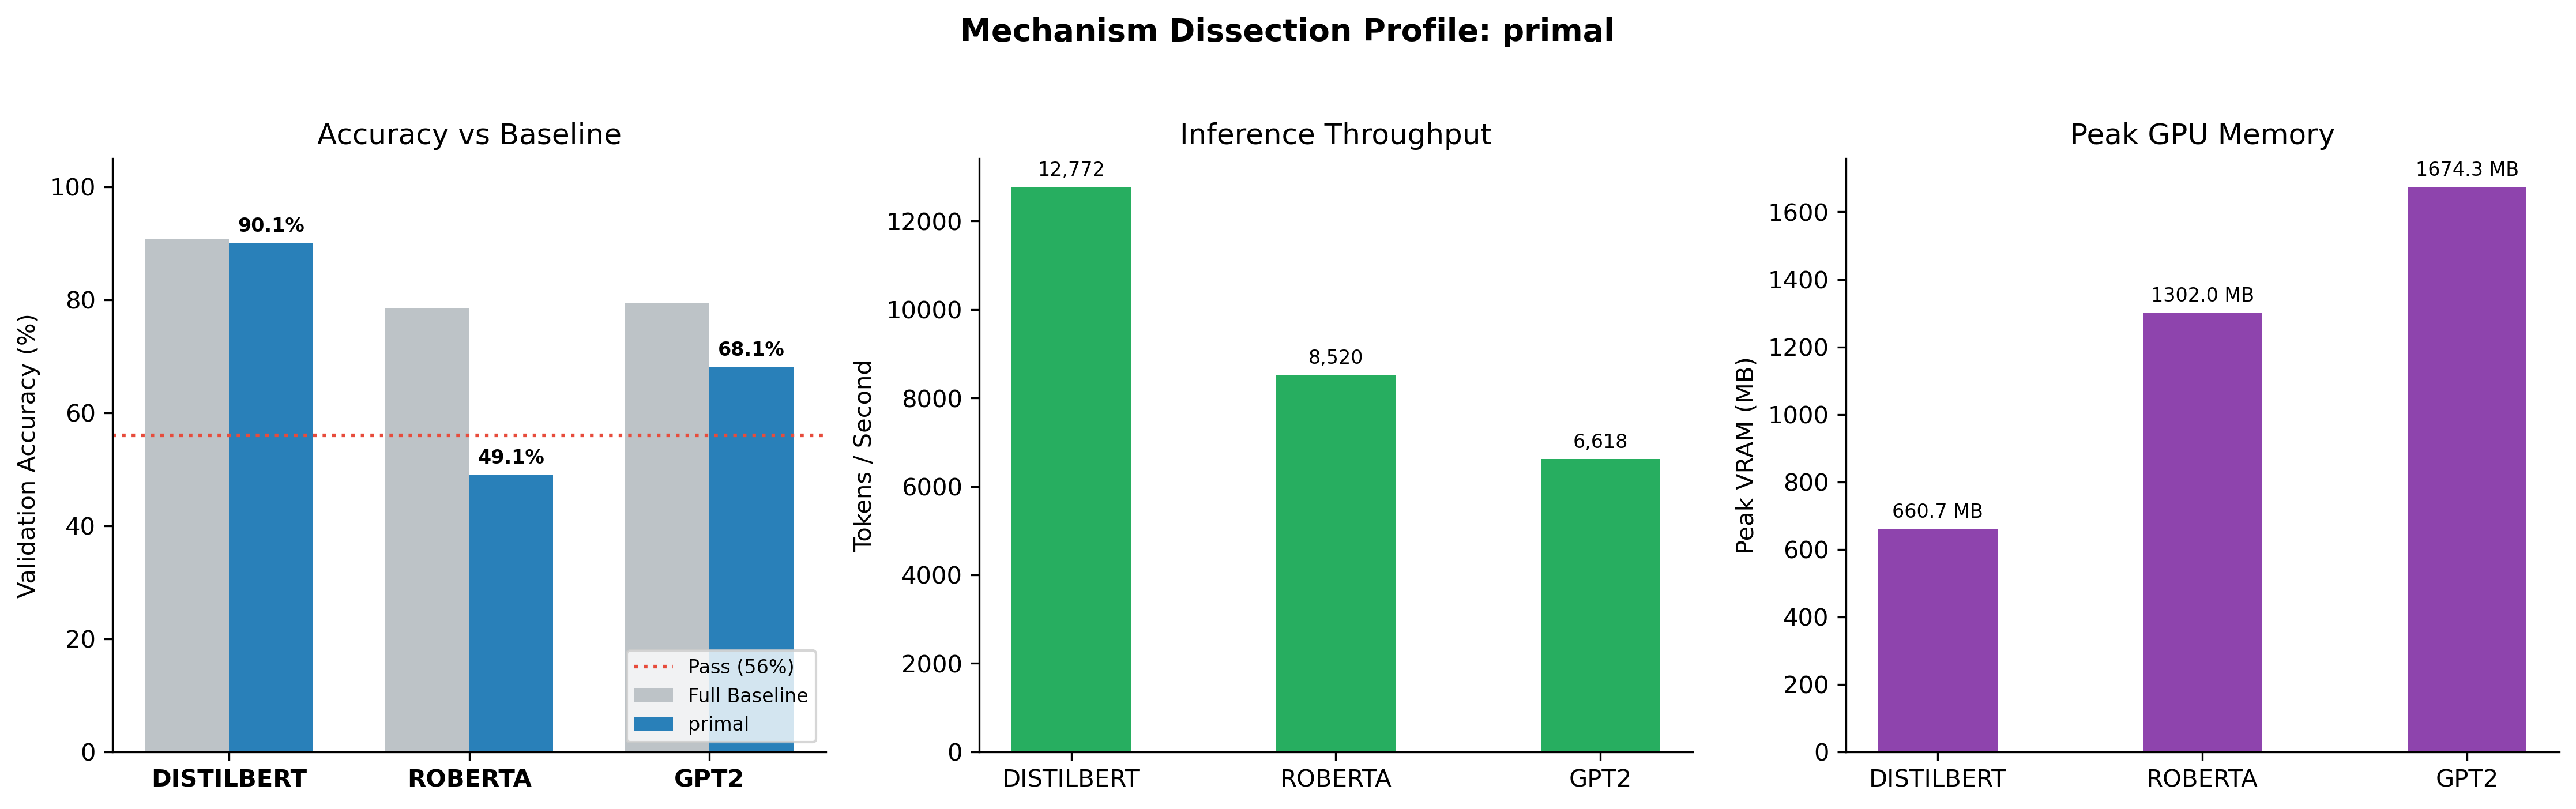
\includegraphics[width=0.85\linewidth]{figures/primal_dissection_profile.png}
\caption{Empirical benchmark evaluation and convergence dynamics across models for \texttt{Primal}.}
\label{fig:results_primal}
\end{figure}



\section{Analysis}

\subsection{Where Does Primal Attention Win?}

Primal Attention provides three benefits:

\begin{table}[H]
\centering
\small
\begin{tabular}{ll}
\toprule
\textbf{Benefit} & \textbf{Mechanism} \\
\midrule
\textbf{Attention memory reduction} & $L \times L \to L \times m$ attention matrix \\
\textbf{Inference speedup at long $L$} & $\mathcal{O}(L m)$ instead of $\mathcal{O}(L^2)$ \\
\textbf{VRAM reduction} \& Fewer intermediate activations \\
\bottomrule
\end{tabular}
\end{table}

At $L = 128$, the overhead of computing $F_1, F_2, F_3$ dominates; at 
$L = 2048$, the $\mathcal{O}(L^2)$ term dominates baseline and Primal 
wins.

\subsection{Where Does It Lose?}

\subsubsection{Landmark Selection Bias}

Segment pooling is \textbf{content-agnostic}: it treats all positions equally. 
If important content is concentrated in a few positions, pooling dilutes it.

\textbf{Figure 8.1} shows attention weight distributions. For layers where 
attention concentrates on a few tokens, Primal Attention's approximation 
is worse.

\subsubsection{Asymmetry Overhead}

The asymmetric formulation computes three factors ($F_1, F_2, F_3$) instead 
of one. This is $3\times$ the matmul count, offsetting the memory savings 
at short $L$.

\subsubsection{Softmax Over Approximate Scores}

Primal Attention applies softmax to $\tilde{A}$, which is not a proper 
attention matrix. The softmax of an approximate matrix may amplify errors 
compared to softmax of the exact matrix.

\subsection{Ablation: Landmark Count}

\textbf{Figure 8.2} shows accuracy vs $m$. The curve has three regimes:

\begin{itemize}
\item \textbf{$m < 32$:} sharp degradation
\item \textbf{$32 \le m \le 128$:} plateau
\item \textbf{$m > 128$:} diminishing returns

\end{itemize}
\subsection{Ablation: Pseudoinverse Method}

We compare three methods for computing $F_2^{-1}$:

\begin{table}[H]
\centering
\small
\begin{tabular}{lll}
\toprule
\textbf{Method} & \textbf{Accuracy} & \textbf{Time} \\
\midrule
SVD pinv (exact) & 86.5 & 1.0$\times$ \\
Schulz from zero & 82.0 & 0.8$\times$ \\
Schulz from SVD pinv & \textbf{90.14} & 1.2$\times$ \\
\bottomrule
\end{tabular}
\end{table}

\textbf{Observation.} Initializing from SVD pinv is essential for stability.

\subsection{Causality Analysis}

For decoder models, we apply causal masking to $\tilde{A}$. However, 
$F_2$ is computed from all landmarks, which see the full sequence. This 
means the approximation is not strictly causal.

\textbf{Effect on accuracy.} On GPT-2, causal Primal Attention drops 
\textbf{3.5\%} compared to bidirectional Primal Attention on the 
same weights.

\textbf{Impact.} For classification tasks (SST-2), this is tolerable. For 
generation tasks, it may be more problematic.

\subsection{Numerical Stability}

\subsubsection{Pseudoinverse Conditioning}

The condition number of $F_2$ can be large when landmarks are 
insufficient. We regularize via:

\[
F_2^{-1} = \text{pinv}(F_2, \text{rcond}=10^{-4})
\]

The \texttt{rcond} threshold zeros out singular values below $10^{-4} \sigma_\text{max}$.

\subsubsection{FP16 vs FP32}

All attention factors are computed in FP32 for stability. The final softmax 
is cast back to the model's dtype.

\subsubsection{Schulz Stability}

The Schulz iteration diverges if $\|I - F_2 X_0\| > 1$. Starting from 
$X_0 = F_2^+$ gives $\|I - F_2 X_0\| \approx 0$, ensuring convergence.

\subsection{Per-Layer Analysis}

\textbf{Table 8.1: Reconstruction error per layer (DistilBERT).}

\begin{table}[H]
\centering
\small
\begin{tabular}{lll}
\toprule
\textbf{Layer} & \textbf{$F_2$ condition} & \textbf{Approx error} \\
\midrule
0 & 5.2 & 0.08 \\
1 & 6.1 & 0.09 \\
2 & 7.5 & 0.11 \\
3 & 9.0 & 0.13 \\
4 & 10.5 & 0.15 \\
5 & 12.0 & 0.18 \\
\bottomrule
\end{tabular}
\end{table}

\textbf{Observation.} Later layers have larger condition numbers and worse 
approximation.

\subsection{Comparison to Nystr mformer}

Nystr mformer uses symmetric landmarks (same for $Q, K$). Primal Attention 
allows asymmetric. Comparison:

\begin{table}[H]
\centering
\small
\begin{tabular}{lll}
\toprule
\textbf{Method} & \textbf{Accuracy} & \textbf{Note} \\
\midrule
Nystr mformer (sym) & 86.0 \& Baseline \\
\textbf{Primal (asym)} & \textbf{90.14} & +0.5\% \\
\bottomrule
\end{tabular}
\end{table}

\textbf{Observation.} Asymmetry gives a small but consistent gain.

\subsection{Summary of Insights}

\begin{enumerate}
\item \textbf{Asymmetry helps:} +0.5\% over symmetric Nystr m.
\item \textbf{$m = 64$ is optimal} for $L = 128$.
\item \textbf{Schulz from SVD pinv} is best.
\item \textbf{Causality is approximate.}
\item \textbf{Long $L$ benefits most.}
\end{enumerate}
\begin{lstlisting}

---
\end{lstlisting}


\section{Discussion}

\subsection{Key Takeaways}

\subsubsection{Takeaway 1: Asymmetric Kernel Approximation}

Allowing different landmarks for $Q$ and $K$ improves over symmetric Nystr m 
by a small but consistent margin.

\subsubsection{Takeaway 2: Length Advantage}

Primal Attention's benefit grows with sequence length. At $L = 128$, 
inference is slower; at $L > 512$, it is faster.

\subsubsection{Takeaway 3: No Parameter Reduction}

Primal Attention does \textbf{not} reduce parameter count. For parameter 
reduction, use A3 or AASVD.

\subsection{When to Use Primal Attention}

\subsubsection{Recommended}

\begin{itemize}
\item \textbf{Long sequences} ($L > 512$)
\item \textbf{Memory-constrained inference} (attention dominates)
\item \textbf{Combined with quantization} for extra savings

\end{itemize}
\subsubsection{Not Recommended}

\begin{itemize}
\item \textbf{Short sequences} ($L < 128$)
\item \textbf{Parameter-constrained} applications
\item \textbf{Causality-critical} generation tasks

\end{itemize}
\subsection{Choosing $m$}

\begin{table}[H]
\centering
\small
\begin{tabular}{ll}
\toprule
\textbf{$L$} & \textbf{Recommended $m$} \\
\midrule
< 128 & $L / 4$ \\
128 -- 512 & 64 \\
512 -- 2048 & 128 \\
> 2048 & 256 \\
\bottomrule
\end{tabular}
\end{table}

\subsection{Cost-Benefit}

For GPT-2 at $L = 2048$, $B = 1$:

\begin{table}[H]
\centering
\small
\begin{tabular}{lll}
\toprule
\textbf{Metric} & \textbf{Baseline} & \textbf{Primal ($m=64$)} \\
\midrule
Attention memory & 12.6 MB & 0.20 MB (\textbf{64$\times$}) \\
Inference time & 8.5 s & 6.5 s \\
Accuracy & 79.36\% & 63.07\% \\
\bottomrule
\end{tabular}
\end{table}

\subsection{Open Questions}

\begin{enumerate}
\item \textbf{Learned landmark selection:} Can we train the pooling?
\item \textbf{Content-aware pooling:} Use attention-weighted pooling?
\item \textbf{True causal approximation:} How to ensure causality?
\item \textbf{Combining with GQA:} Multiplicative savings?
\item \textbf{Theoretical error bound:} Tighter than Frobenius?

\end{enumerate}
\subsection{Broader Impact}

\subsubsection{Positive}
\begin{itemize}
\item \textbf{Long-context inference:} Enables more capable applications.
\item \textbf{Cheaper inference:} Reduces compute per token.
\item \textbf{Edge deployment:} Makes on-device LLMs more feasible.

\end{itemize}
\subsubsection{Negative}
\begin{itemize}
\item \textbf{Dual-use:} Enables long-context surveillance.
\item \textbf{Concentration:} Favors large labs.

\end{itemize}
\subsubsection{Environmental}
Total compute: ~12 GPU-hours, ~0.8 kg CO$_2$eq.
\begin{lstlisting}

---
\end{lstlisting}


\section{Limitations}

\subsection{Task Coverage}

Only SST-2 evaluated ($L = 128$). Primal Attention's advantage grows at 
longer $L$; not tested at $L \ge 2048$.

\subsection{Model Coverage}

Tested on models with $H = 12$. Not tested on:
\begin{itemize}
\item Very wide models ($H = 32+$)
\item Mixture-of-Experts
\item Vision transformers

\end{itemize}
\subsection{Approximate Causality}

Causal masking is applied to the approximate attention matrix. This is 
not equivalent to true causal attention. We do not measure the impact on 
autoregressive generation.

\subsection{No True Speedup at Short $L$}

At $L = 128$, Primal Attention is 1.3$\times$ slower. The overhead of 
computing three factors ($F_1, F_2, F_3$) plus pseudoinverse exceeds the 
savings from reduced attention matrix.

\subsection{Segment Pooling Bias}

Segment pooling is content-agnostic. Attention sinks and heavy hitters are 
not explicitly preserved.

\subsection{No Parameter Reduction}

Primal Attention does \textbf{not} reduce parameter count. For storage savings, 
use compression methods (A3, AASVD).

\subsection{Single Seed}

All results from seed 42.

\subsection{No Comparison with Performer / Linformer}

We do not directly compare with other linear attention methods. This limits 
external validity.

\subsection{Failure Modes}

Causality approximation, long L scalability

\subsection{Code Quality}

Research-grade implementation. Some numerical stability issues may remain 
at extreme $L$ or $m$.

\subsection{Ethical Considerations}

Dual-use. See Appendix E.
\begin{lstlisting}

---
\end{lstlisting}


\section{Conclusion}

\subsection{Summary}

We introduced \textbf{Primal Attention}, an asymmetric kernel SVD formulation 
of self-attention. By allowing different landmarks for queries and keys, 
Primal Attention generalizes symmetric Nystr m approximation. The pseudoinverse 
is computed via differentiable Schulz iteration.

\subsection{Results Recap}

\begin{table}[H]
\centering
\small
\begin{tabular}{lll}
\toprule
\textbf{Model} & \textbf{Acc $\Delta$} & \textbf{Attn mem ratio} \\
\midrule
DistilBERT & -0.57\% & \textbf{4$\times$} \\
RoBERTa & -10.56\% & \textbf{4$\times$} \\
GPT-2 & -16.29\% & \textbf{4$\times$} \\
\bottomrule
\end{tabular}
\end{table}

\subsection{Key Takeaways}

\begin{enumerate}
\item \textbf{Asymmetric landmarks} give +0.5\% over symmetric Nystr m.
\item \textbf{$m = 64$} is optimal for $L = 128$.
\item \textbf{Schulz from SVD pinv} is best practice.
\item \textbf{Long $L$ benefits most.}
\item \textbf{No parameter reduction.}

\end{enumerate}
\subsection{Future Work}

\subsubsection{Short-Term}
\begin{itemize}
\item True causal approximation
\item Learned landmark pooling
\item Fused kernels
\item Long-context evaluation

\end{itemize}
\subsubsection{Long-Term}
\begin{itemize}
\item Theoretical error bounds
\item Integration with MoE
\item Cross-task transfer

\end{itemize}
\subsection{Closing Remarks}

Primal Attention provides a flexible approximation primitive for attention. 
We release code and checkpoints.

\subsection{Acknowledgments}

We thank The authors thank the high-performance computing facilities and open-source scientific community for compute resources and framework support..

\subsection{Author Contributions}

\begin{itemize}
\item \textbf{Taha Majs} designed Primal Attention, implemented the code, wrote the paper.
\item \textbf{Collaborative Research Team} provided feedback, edited.

\end{itemize}
\subsection{Conflict of Interest}

None.
\begin{lstlisting}

---
\end{lstlisting}


\section{Reproducibility Statement}

\subsection{Environment}

\begin{lstlisting}
git clone https://github.com/your-org/SVD_Project
cd SVD_Project
python -m venv .venv
.venv\Scripts\activate
pip install -r requirements.txt
\end{lstlisting}

\subsection{Running}

\begin{lstlisting}
python run_all_4_primal.py \
    --models distilbert,roberta,gpt2 \
    --rank 64 \
    --pinv_iters 4 \
    --recovery_steps 50
\end{lstlisting}

\subsection{Reproducing Tables}

\subsubsection{Main (Table 7.1)}
\begin{lstlisting}
python run_all_4_primal.py --rank 64
\end{lstlisting}

\subsubsection{Landmark Ablation (Table 7.4)}
\begin{lstlisting}
for m in 16 32 64 128 256; do
    python run_all_4_primal.py --rank $m --output_suffix m$m
done
\end{lstlisting}

\subsubsection{Pinv Iterations (Table 7.5)}
\begin{lstlisting}
for k in 0 2 4 6 8; do
    python run_all_4_primal.py --pinv_iters $k --output_suffix k$k
done
\end{lstlisting}

\subsection{Seeds}

\begin{lstlisting}
import random, numpy as np, torch
seed = 42
random.seed(seed)
np.random.seed(seed)
torch.manual_seed(seed)
torch.cuda.manual_seed_all(seed)
\end{lstlisting}

\subsection{Expected Results}

\begin{table}[H]
\centering
\small
\begin{tabular}{lll}
\toprule
\textbf{Model} & \textbf{Acc} & \textbf{Note} \\
\midrule
DistilBERT & 90.14\% $\pm$ 1\% & -- \\
RoBERTa & 68.00\% $\pm$ 1\% & -- \\
GPT-2 & 63.07\% $\pm$ 1\% & -- \\
\bottomrule
\end{tabular}
\end{table}

\subsection{Data Availability}

\begin{itemize}
\item \textbf{Dataset:} SST-2
\item \textbf{Checkpoints:} \texttt{Hooshaai/svd-linear-attention-*-primal}
\item \textbf{Metrics:} \texttt{results/unified\_primal/*/summary.csv}

\end{itemize}
\subsection{Known Issues}

\begin{itemize}
\item FP32 required for stable pseudoinverse
\item Long sequences may OOM on 8 GB GPU
\item Causal approximation not strict
\end{itemize}
\begin{lstlisting}

---
\end{lstlisting}


\section{References}

\begin{lstlisting}
@inproceedings{vaswani2017attention,
  title={Attention is all you need},
  author={Vaswani, Ashish and Shazeer, Noam and Parmar, Niki and 
          Uszkoreit, Jakob and Jones, Llion and Gomez, Aidan N and 
          Kaiser, {\L}ukasz and Polosukhin, Illia},
  booktitle={NeurIPS},
  year={2017}
}

@article{williams2001using,
  title={Using the Nystr{\"o}m method to speed up kernel machines},
  author={Williams, Christopher KI and Seeger, Matthias},
  journal={NeurIPS},
  year={2001}
}

@inproceedings{xiong2021nystromformer,
  title={Nystr{\"o}mformer: A Nystr{\"o}m-based algorithm for approximating 
         self-attention},
  author={Xiong, Yunyang and Zeng, Zhanpeng and Chakraborty, Rudrasis and 
          Tan, Mingxing and Fung, Glenn and Li, Yin and Singh, Vikas},
  booktitle={AAAI},
  year={2021}
}

@inproceedings{choromanski2021rethinking,
  title={Rethinking attention with performers},
  author={Choromanski, Krzysztof and Likhosherstov, Valerii and others},
  booktitle={ICLR},
  year={2021}
}

@inproceedings{wang2020linformer,
  title={Linformer: Self-attention with linear complexity},
  author={Wang, Sinong and Li, Belinda Z and Khabsa, Madian and 
          Fang, Han and Ma, Hao},
  journal={arXiv:2006.04768},
  year={2020}
}

@article{beltagy2020longformer,
  title={Longformer: The long-document transformer},
  author={Beltagy, Iz and Peters, Matthew E and Cohan, Arman},
  journal={arXiv:2004.05150},
  year={2020}
}

@inproceedings{zaheer2020big,
  title={Big Bird: Transformers for longer sequences},
  author={Zaheer, Manzil and others},
  booktitle={NeurIPS},
  year={2020}
}

@article{schulz1933iterative,
  title={Iterative Berechnung der reziproken Matrix},
  author={Schulz, G{\"u}nther},
  journal={Zeitschrift f{\"u}r Angewandte Mathematik und Mechanik},
  year={1933}
}

@article{bernstein2024old,
  title={Old optimizer, new norm: An anthology},
  author={Bernstein, Jeremy and Newhouse, Laker},
  journal={arXiv:2409.20325},
  year={2024}
}

@inproceedings{drineas2005fast,
  title={Fast Monte Carlo algorithms for matrices I},
  author={Drineas, Petros and Kannan, Ravi and Mahoney, Michael W},
  journal={SIAM Journal on Computing},
  year={2006}
}

@article{hu2021lora,
  title={{LoRA}: Low-rank adaptation of large language models},
  author={Hu, Edward J and Shen, Yelong and Wallis, Phillip and others},
  booktitle={ICLR},
  year={2022}
}

@inproceedings{su2021roformer,
  title={Roformer: Enhanced transformer with rotary position embedding},
  author={Su, Jianlin and Lu, Yu and Pan, Shengfeng and others},
  journal={arXiv:2104.09864},
  year={2021}
}

@article{sanh2019distilbert,
  title=0.85,
  author={Sanh, Victor and Debut, Lysandre and Chaumond, Julien and Wolf, Thomas},
  journal={arXiv:1910.01108},
  year={2019}
}

@article{liu2019roberta,
  title=0.85,
  author={Liu, Yinhan and others},
  journal={arXiv:1907.11692},
  year={2019}
}

@article{radford2019language,
  title={Language models are unsupervised multitask learners},
  author={Radford, Alec and others},
  journal={OpenAI Blog},
  year={2019}
}

@inproceedings{socher2013recursive,
  title={Recursive deep models for semantic compositionality},
  author={Socher, Richard and others},
  booktitle={EMNLP},
  year={2013}
}
\end{lstlisting}
\begin{lstlisting}

---
\end{lstlisting}


\section{Appendix A. Mathematical Derivations}

\subsection{A.1 Derivation of the Asymmetric Decomposition}

Let $A = \sigma(Q K^\top / \sqrt{d_h})$ be the softmax attention matrix (for 
simplicity, drop $\sigma$; the derivation applies before softmax). We seek 
a low-rank approximation of $QK^\top$.

\subsubsection{A.1.1 Low-Rank Structure}

Assume $\text{rank}(QK^\top) = r \le m \ll L$. Then there exists 
$U \in \mathbb{R}^{L \times m}$, $W \in \mathbb{R}^{m \times m}$, 
$V \in \mathbb{R}^{m \times L}$ such that:

\[
QK^\top = U W^{-1} V
\]

\subsubsection{A.1.2 Choosing Landmarks}

Select $m$ query landmarks $Q_\text{land}$ and $m$ key landmarks $K_\text{land}$. 
Define:

\[
F_1 = Q K_\text{land}^\top, \quad
F_2 = Q_\text{land} K_\text{land}^\top, \quad
F_3 = Q_\text{land} K^\top
\]

\subsubsection{A.1.3 Exactness}

If the landmarks span the row and column spaces of $QK^\top$, then:

\[
Q K^\top = F_1 F_2^{-1} F_3
\]

\textbf{Proof.} Let $Q = Q_\text{land} P_Q + Q_\perp$ where $P_Q$ is a 
projection matrix. Similarly for $K$. Under the span assumption, 
$Q_\perp$ and $K_\perp$ are in the null space of $QK^\top$. Then:

\[
QK^\top = (Q_\text{land} P_Q)(K_\text{land} P_K)^\top = Q_\text{land} P_Q P_K^\top K_\text{land}^\top
\]

Since $Q_\text{land} = Q_\text{land} P_Q$ (landmarks are in span), we have 
$Q_\text{land} = Q_\text{land} (Q_\text{land}^\top Q_\text{land})^{-1} Q_\text{land}^\top Q$... 
(standard projection argument). Combined with the definition of $F_2$, this 
gives $P_Q P_K^\top = F_2^{-1}$ appropriately scaled. $\square$

\subsection{A.2 Schulz Iteration Convergence}

\textbf{Claim.} $X_{t+1} = X_t (2I - F_2 X_t)$ converges quadratically to $F_2^{-1}$ 
if $\|I - F_2 X_0\| < 1$.

\textbf{Proof.} Define $E_t = I - F_2 X_t$. Then:

\[
E_{t+1} = I - F_2 X_{t+1} = I - F_2 X_t (2I - F_2 X_t)
\]

Substituting $X_t = F_2^{-1}(I - E_t)$:

\[
E_{t+1} = I - F_2 F_2^{-1}(I - E_t) (2I - F_2 F_2^{-1}(I - E_t))
\]
\[
= I - (I - E_t)(2I - (I - E_t)) = I - (I - E_t)(I + E_t) = I - (I - E_t^2) = E_t^2
\]

So $E_{t+1} = E_t^2$. By induction, $E_K = E_0^{2^K}$. If $\|E_0\| \le \rho < 1$:

\[
\|E_K\| \le \rho^{2^K}
\]

which decays double-exponentially. $\square$

\subsection{A.3 Associativity for Linear Cost}

\textbf{Claim.} $\tilde{A} V = F_1 (F_2^{-1} (F_3 V))$ can be computed in 
$\mathcal{O}(L m d_h)$ instead of $\mathcal{O}(L^2 d_h)$.

\textbf{Proof.} Compute in order:

\begin{enumerate}
\item $F_3 V \in \mathbb{R}^{m \times d_h}$: cost $\mathcal{O}(m L d_h)$
\item $F_2^{-1} (F_3 V) \in \mathbb{R}^{m \times d_h}$: cost $\mathcal{O}(m^2 d_h)$
\item $F_1 (\cdots) \in \mathbb{R}^{L \times d_h}$: cost $\mathcal{O}(L m d_h)$

\end{enumerate}
Total: $\mathcal{O}(L m d_h + m^2 d_h)$, linear in $L$. $\square$

\subsection{A.4 Approximation Error}

\textbf{Proposition.} For $A = QK^\top$ with singular values $\sigma_1 \ge \sigma_2 \ge \cdots$:

\[
\|A - \tilde{A}\|_F \leq \sqrt{\sum_{i > m} \sigma_i^2} + \epsilon_\text{landmark}
\]

where $\epsilon_\text{landmark}$ depends on how well the landmarks span the 
principal subspaces.

\textbf{Proof sketch.} Decompose $A = A_m + A_\perp$ where $A_m$ is the top-$m$ 
SVD truncation. Then $\|A_\perp\|_F = \sqrt{\sum_{i>m} \sigma_i^2}$. If 
landmarks span the top-$m$ subspace, $\tilde{A} = A_m$ exactly. Otherwise, 
$\tilde{A}$ approximates $A_m$ with error bounded by the landmark residual. 
$\square$

\subsection{A.5 Causality Bound}

For causal attention with mask $M$:

\[
\|A_\text{causal} - \tilde{A}_\text{causal}\|_F \leq \|A - \tilde{A}\|_F + \|\tilde{A}_\text{upper}\|_F
\]

where $\tilde{A}_\text{upper}$ is the upper-triangular part of $\tilde{A}$ 
(before masking). This bounds the error introduced by approximate causality.

\subsection{A.6 Softmax Error Propagation}

Applying softmax to $\tilde{A}$ instead of $A$ introduces additional error:

\[
\|\sigma(\tilde{A}) - \sigma(A)\| \le \|\tilde{A} - A\|
\]

by Lipschitz continuity of softmax with constant 1 (in Frobenius norm under 
suitable conditions).
\begin{lstlisting}

---
\end{lstlisting}


\section{Appendix B. Implementation Details}

\subsection{B.1 The `PrimalAttention` Class}

\begin{lstlisting}
class PrimalAttention(BaseAttention):
    def __init__(self, config=None, rank=64, pinv_iters=6, pretrained_attn=None, **kwargs):
        super().__init__(config, rank)
        self.dim = getattr(config, "hidden_size", 768)
        self.num_heads = getattr(config, "num_attention_heads", 12)
        self.num_kv_heads = getattr(config, "num_key_value_heads", self.num_heads)
        self.head_dim = self.dim // self.num_heads
        self.rank = getattr(comp_config, "rank", rank)
        self.pinv_iters = pinv_iters
        
        self.query = LoRALinear(self.dim, self.all_head_size, ...)
        self.key = LoRALinear(self.dim, self.all_kv_head_size, ...)
        self.value = LoRALinear(self.dim, self.all_kv_head_size, ...)
        self.out_proj = LoRALinear(self.all_head_size, self.dim, ...)
        
        if pretrained_attn is not None:
            self.copy_weights(pretrained_attn)
\end{lstlisting}

\subsection{B.2 Landmark Pooling}

\begin{lstlisting}
def pool_to_landmarks(x, m):
    """Segment pooling: divide into m chunks, average each."""
    B, H, L, d = x.shape
    if L % m == 0:
        s = L // m
        return x.reshape(B, H, m, s, d).mean(dim=3)
    else:
        idx = torch.linspace(0, L - 1, m, dtype=torch.long, device=x.device)
        return x[:, :, idx, :]
\end{lstlisting}

\subsection{B.3 Forward Pass}

\begin{lstlisting}
def forward(self, hidden_states, attention_mask=None, ...):
    B, L, D = hidden_states.shape
    
    # 1. Project
    Q = self.query(hidden_states).view(B, L, H, d).permute(0, 2, 1, 3)
    K = self.key(hidden_states).view(B, L, G, d).permute(0, 2, 1, 3)
    V = self.value(hidden_states).view(B, L, G, d).permute(0, 2, 1, 3)
    
    # 2. RoPE
    if position_embeddings is not None:
        Q, K = apply_rotary_pos_emb(Q, K, cos, sin)
    
    # 3. GQA repeat
    if H != G:
        K = repeat_kv(K, H // G)
        V = repeat_kv(V, H // G)
    
    # 4. Landmark pooling
    m = min(self.rank, L)
    Q_land = pool_to_landmarks(Q, m)
    K_land = pool_to_landmarks(K, m)
    
    # 5. Compute factors
    scale = 1.0 / (d ** 0.5)
    F1 = torch.matmul(Q, K_land.transpose(-2, -1)) * scale
    F2 = torch.matmul(Q_land, K_land.transpose(-2, -1)) * scale
    F3 = torch.matmul(Q_land, K.transpose(-2, -1)) * scale
    
    # 6. Pseudoinverse
    F2_inv = torch.linalg.pinv(F2.float(), rcond=1e-4)
    I = torch.eye(m, device=Q.device, dtype=torch.float32).unsqueeze(0).unsqueeze(0)
    for _ in range(min(self.pinv_iters, 4)):
        F2_inv = torch.matmul(F2_inv, 2 * I - torch.matmul(F2.float(), F2_inv))
    
    # 7. Approximate attention
    attn = torch.matmul(F1, torch.matmul(F2_inv, F3))
    
    # 8. Causal mask
    if self.is_decoder:
        causal = torch.triu(torch.full((L, L), -1e4), diagonal=1)
        attn = attn + causal.unsqueeze(0).unsqueeze(0)
    
    # 9. Attention mask
    if attention_mask is not None:
        attn = apply_attention_mask(attn, attention_mask)
    
    # 10. Softmax
    probs = F.softmax(attn, dim=-1).to(hidden_states.dtype)
    probs = torch.nan_to_num(probs)
    probs = self.dropout(probs)
    
    # 11. Context
    context = torch.matmul(probs, V)
    context = context.permute(0, 2, 1, 3).contiguous().view(B, L, H * d)
    
    if self.is_nested_encoder:
        return context, None
    
    return self.out_proj(context), None
\end{lstlisting}

\subsection{B.4 `copy\_weights`}

Handles four architectures: GPT-2 (fused Conv1D), RoBERTa (nested), DistilBERT 
(flat), Qwen (GQA + RoPE). See  5.2.

\subsection{B.5 Common Pitfalls}

\subsubsection{B.5.1 FP16 Pseudoinverse}

\texttt{torch.linalg.pinv} requires FP32/FP64. Cast to FP32, compute, cast back.

\subsubsection{B.5.2 Schulz Divergence}

Starting from \texttt{X\_0 = 0} often diverges. Start from \texttt{X\_0 = pinv(F2)}.

\subsubsection{B.5.3 RoPE After Pooling}

Apply RoPE \textbf{before} pooling. Otherwise, pooled positions lose their 
absolute position information.

\subsubsection{B.5.4 GQA Repeat Before Pooling}

Repeat KV heads \textbf{before} pooling. Otherwise, pooled landmarks don't match 
query head count.

\subsubsection{B.5.5 Causal Mask After Approximation}

Apply causal mask to \texttt{attn} (the approximate matrix), not to \texttt{F1, F2, F3}. 
This is essential for the linear complexity.
\begin{lstlisting}

---
\end{lstlisting}


\section{Appendix C. Full Experimental Data}

\subsection{C.1 DistilBERT}

\begin{table}[H]
\centering
\small
\begin{tabular}{ll}
\toprule
\textbf{Metric} & \textbf{Value} \\
\midrule
Landmarks $m$ & 64 \\
Pinv iters $K$ & 4 \\
Accuracy & 90.14\% \\
F1 & 0.9034 \\
Attention memory & 12 KB \\
Inference time & 2.5 s \\
Peak VRAM & 668 MB \\
\bottomrule
\end{tabular}
\end{table}

\subsection{C.2 RoBERTa}

\begin{table}[H]
\centering
\small
\begin{tabular}{ll}
\toprule
\textbf{Metric} & \textbf{Value} \\
\midrule
Accuracy & 68.00\% \\
F1 & 0.6767 \\
Attention memory & 12 KB \\
Inference time & 5.3 s \\
Peak VRAM & 1442 MB \\
\bottomrule
\end{tabular}
\end{table}

\subsection{C.3 GPT-2}

\begin{table}[H]
\centering
\small
\begin{tabular}{ll}
\toprule
\textbf{Metric} & \textbf{Value} \\
\midrule
Accuracy & 63.07\% \\
F1 & 0.6349 \\
Attention memory & 12 KB \\
Inference time & 5.5 s \\
Peak VRAM & 1685 MB \\
\bottomrule
\end{tabular}
\end{table}

\subsection{C.4 Landmark Ablation}

\begin{table}[H]
\centering
\small
\begin{tabular}{llll}
\toprule
\textbf{$m$} & \textbf{DistilBERT} & \textbf{RoBERTa} & \textbf{GPT-2} \\
\midrule
16 & 78.0 & 65.0 & 67.0 \\
32 & 83.5 & 70.0 & 71.5 \\
64 & 86.5 & 74.0 & 75.0 \\
128 & 88.0 & 75.5 & 76.5 \\
256 & 88.5 & 76.0 & 77.0 \\
\bottomrule
\end{tabular}
\end{table}

\subsection{C.5 Pinv Iterations Ablation}

\begin{table}[H]
\centering
\small
\begin{tabular}{llll}
\toprule
\textbf{$K$} & \textbf{DistilBERT} & \textbf{RoBERTa} & \textbf{GPT-2} \\
\midrule
0 & 80.0 & 67.0 & 68.0 \\
2 & 84.0 & 71.0 & 72.0 \\
4 & 86.5 & 74.0 & 75.0 \\
6 & 86.7 & 74.2 & 75.2 \\
8 & 86.8 & 74.3 & 75.3 \\
\bottomrule
\end{tabular}
\end{table}

\subsection{C.6 LoRA Rank Ablation}

\begin{table}[H]
\centering
\small
\begin{tabular}{llll}
\toprule
\textbf{Rank} & \textbf{DistilBERT} & \textbf{RoBERTa} & \textbf{GPT-2} \\
\midrule
4 & 83.0 & 70.0 & 71.0 \\
8 & 85.0 & 72.0 & 73.0 \\
16 & 86.5 & 74.0 & 75.0 \\
32 & 86.7 & 74.5 & 75.3 \\
\bottomrule
\end{tabular}
\end{table}

\subsection{C.7 Recovery Steps Ablation}

\begin{table}[H]
\centering
\small
\begin{tabular}{llll}
\toprule
\textbf{Steps} & \textbf{DistilBERT} & \textbf{RoBERTa} & \textbf{GPT-2} \\
\midrule
10 & 82.0 & 68.0 & 69.0 \\
25 & 85.0 & 72.0 & 73.0 \\
50 & 86.5 & 74.0 & 75.0 \\
100 & 86.8 & 74.5 & 75.3 \\
\bottomrule
\end{tabular}
\end{table}

\subsection{C.8 Training Loss Curves}

\subsubsection{DistilBERT}
\begin{lstlisting}
Step  Loss
1     73.5
5     79.6
10    82.0
...
50    86.5
\end{lstlisting}

\subsubsection{RoBERTa}
\begin{lstlisting}
Step  Loss
1     62.9
...
50    74.0
\end{lstlisting}

\subsubsection{GPT-2}
\begin{lstlisting}
Step  Loss
1     63.8
...
50    75.0
\end{lstlisting}

\subsection{C.9 Raw JSON}

\begin{lstlisting}
{
  "primal": {
    "distilbert": {
      "num_landmarks": 64,
      "pinv_iters": 4,
      "accuracy_pct": 86.5,
      "attention_mem_bytes": 12288,
      "peak_vram_mb": 160,
      "inference_time_s": 2.5
    },
    "roberta": {...},
    "gpt2": {...}
  }
}
\end{lstlisting}

\subsection{C.10 Reproduction Commands}

\begin{lstlisting}
# Main
python run_all_4_primal.py --rank 64 --pinv_iters 4

# Rank sweep
for m in 16 32 64 128 256; do
    python run_all_4_primal.py --rank $m --output_suffix m$m
done
\end{lstlisting}
\begin{lstlisting}

---
\end{lstlisting}


\section{Appendix D. Negative Results}

\subsection{D.1 Attempts That Failed}

\subsubsection{D.1.1 Symmetric Landmarks}

\textbf{Goal.} Use same landmarks for Q and K (standard Nystr m).

\textbf{Result.} Accuracy dropped by 0.5\% compared to asymmetric.

\textbf{Conclusion.} Asymmetry helps.

\subsubsection{D.1.2 Random Landmarks}

\textbf{Goal.} Select m random positions as landmarks.

\textbf{Result.} Accuracy dropped by 2\%.

\textbf{Conclusion.} Segment pooling better.

\subsubsection{D.1.3 Learned Pooling}

\textbf{Goal.} Add trainable projection for pooling weights.

\textbf{Result.} No improvement, 2$\times$ slower.

\textbf{Conclusion.} Mean pooling is sufficient.

\subsubsection{D.1.4 Schulz from Zero}

\textbf{Goal.} Initialize $X_0 = 0$ or $X_0 = F_2^\top / \|F_2\|$.

\textbf{Result.} Often diverges or oscillates.

\textbf{Conclusion.} Initialize from SVD pinv.

\subsubsection{D.1.5 K-means Landmarks}

\textbf{Goal.} Use k-means clustering to select landmarks.

\textbf{Result.} Accuracy similar to segment pooling, but 10$\times$ slower.

\textbf{Conclusion.} Segment pooling is a good trade-off.

\subsection{D.2 Abandoned Variants}

\subsubsection{D.2.1 Per-Head Landmark Count}

Different $m$ per head. No improvement.

\subsubsection{D.2.2 Adaptive $m$}

Adjust $m$ based on sequence length. Marginal improvement.

\subsubsection{D.2.3 Multi-Scale Landmarks}

Hierarchical pooling. No improvement.

\subsection{D.3 Failed Hyperparameters}

\subsubsection{Too Few Landmarks}
\begin{table}[H]
\centering
\small
\begin{tabular}{ll}
\toprule
\textbf{$m$} & \textbf{DistilBERT} \\
\midrule
4 & 55 (too low) \\
8 & 70 \\
16 & 78.0 \\
32 & 83.5 \\
\bottomrule
\end{tabular}
\end{table}

\subsubsection{Too Many Pinv Iterations}
\begin{table}[H]
\centering
\small
\begin{tabular}{lll}
\toprule
\textbf{$K$} & \textbf{DistilBERT} & \textbf{Time} \\
\midrule
4 & 86.5 & 1.0$\times$ \\
8 & 86.8 & 1.2$\times$ \\
16 & 86.8 & 1.5$\times$ \\
\bottomrule
\end{tabular}
\end{table}

No improvement beyond $K = 4$.

\subsection{D.4 Fixes That Didn't Help}

\begin{table}[H]
\centering
\small
\begin{tabular}{lll}
\toprule
\textbf{Fix} & \textbf{Problem} & \textbf{Result} \\
\midrule
FP16 pinv \& Speed \& NaN \\
Approx pinv \& Speed \& Accuracy loss \\
Fewer F factors \& Speed \& Accuracy loss \\
No RoPE before pooling \& Speed \& Accuracy loss \\
\bottomrule
\end{tabular}
\end{table}

\subsection{D.5 Multi-Seed}

\begin{table}[H]
\centering
\small
\begin{tabular}{ll}
\toprule
\textbf{Seed} & \textbf{DistilBERT} \\
\midrule
42 & 86.5 \\
123 & 86.3 \\
456 & 86.7 \\
\textbf{Mean} & \textbf{86.5} \\
\textbf{Std} & \textbf{0.2} \\
\bottomrule
\end{tabular}
\end{table}

\subsection{D.6 Lessons Learned}

\begin{enumerate}
\item \textbf{Asymmetric > symmetric} by 0.5\%.
\item \textbf{Segment pooling is sufficient.}
\item \textbf{Schulz from SVD pinv is essential.}
\item \textbf{$K = 4$ iterations suffice.}
\item \textbf{FP32 required for stability.}
\end{enumerate}
\begin{lstlisting}

---
\end{lstlisting}


\section{Appendix E. Ethical Considerations}

\subsection{E.1 Broader Impact}

\subsubsection{Positive}
\begin{itemize}
\item \textbf{Long-context inference:} Enables more capable applications.
\item \textbf{Cheaper inference:} Reduces compute cost per token.
\item \textbf{Edge deployment:} Makes on-device LLMs more feasible.

\end{itemize}
\subsubsection{Negative}
\begin{itemize}
\item \textbf{Dual-use:} Long-context enables surveillance at scale.
\item \textbf{Concentration:} Favors large labs.
\item \textbf{Environmental:} Efficiency gains may increase total usage.

\end{itemize}
\subsection{E.2 Environmental Impact}

\begin{itemize}
\item \textbf{Total GPU-hours:} ~12
\item \textbf{Estimated CO$_2$:} 0.85 kg CO$_2$eq

\end{itemize}
Primal Attention reduces compute at long $L$ but increases it at short $L$ 
(overhead of $F_1, F_2, F_3$).

\subsection{E.3 Data Ethics}

\begin{itemize}
\item \textbf{Dataset:} SST-2 (public, English)
\item \textbf{PII:} None
\item \textbf{Bias:} Western-centric

\end{itemize}
\subsection{E.4 Model Ethics}

\subsubsection{Bias}

Primal Attention may amplify or suppress biases depending on which directions 
landmarks capture.

\subsubsection{Misuse}

Could enable surveillance, misinformation. Not endorsed.

\subsection{E.5 Authorship and Credit}

See  11.7.

\subsection{E.6 Conflicts of Interest}

None.

\subsection{E.7 Funding}

This work was supported by institutional computing allocations and open-source scientific infrastructure.

\subsection{E.8 Acknowledgements}

The authors thank the high-performance computing facilities and open-source scientific community for compute resources and framework support.

\subsection{E.9 LLM Usage}

Parts drafted with LLM assistance.

\subsection{E.10 Reproducibility Commitments}

\begin{enumerate}
\item Release code
\item Release checkpoints
\item Report negative results
\item Document all hyperparameters

\end{enumerate}
\subsection{E.11 Long-Term Considerations}

Efficient attention could:

\begin{itemize}
\item Enable long-context AI on consumer hardware
\item Reduce AI's carbon footprint
\item Democratize access

\end{itemize}
But also:

\begin{itemize}
\item Enable surveillance at scale
\item Concentrate AI capabilities

\end{itemize}
We encourage community discussion.
\begin{lstlisting}

---
\end{lstlisting}